\chapter{Introduction}\label{sec:introduction}

\section{Motivation}\label{sec:motivation}
Aerial imagery is an important resource for applications that include urban planning and map-making~\cite{5523977}.
Ribbon-like features such as sidewalks, street networks, canals, or biking paths are thin thin structures with a medial
curve and varying width. They are especially important because they provide essential connections between sites to
support transportation of people and materials. Any damage or obstacle that appears on these ribbon-like features may
interfere with the navigability of the walking path and could even cause harm to people. High-resolution aerial imagery
has become a way to capture the appearance of these structures in order to look for changes such as new construction,
degradation, damage, or obstructions. Geometrically, walking paths are thin features that can be described by a
trajectory with varying thickness~\cite{10.1007/11744078_9}. The scope of this thesis is automatic refinement of
ribbon-like features: given an approximate trajectory and range of potential thicknesses, we automate the process of
estimating the thicknesses and offset of the trajectory. One example of a downstream application is to enable accurate
walking instructions for people including those with disabilities detect and avoid obstacles such as stairways~\cite{ZOU2012227}.

\begin{figure} 
\centering 
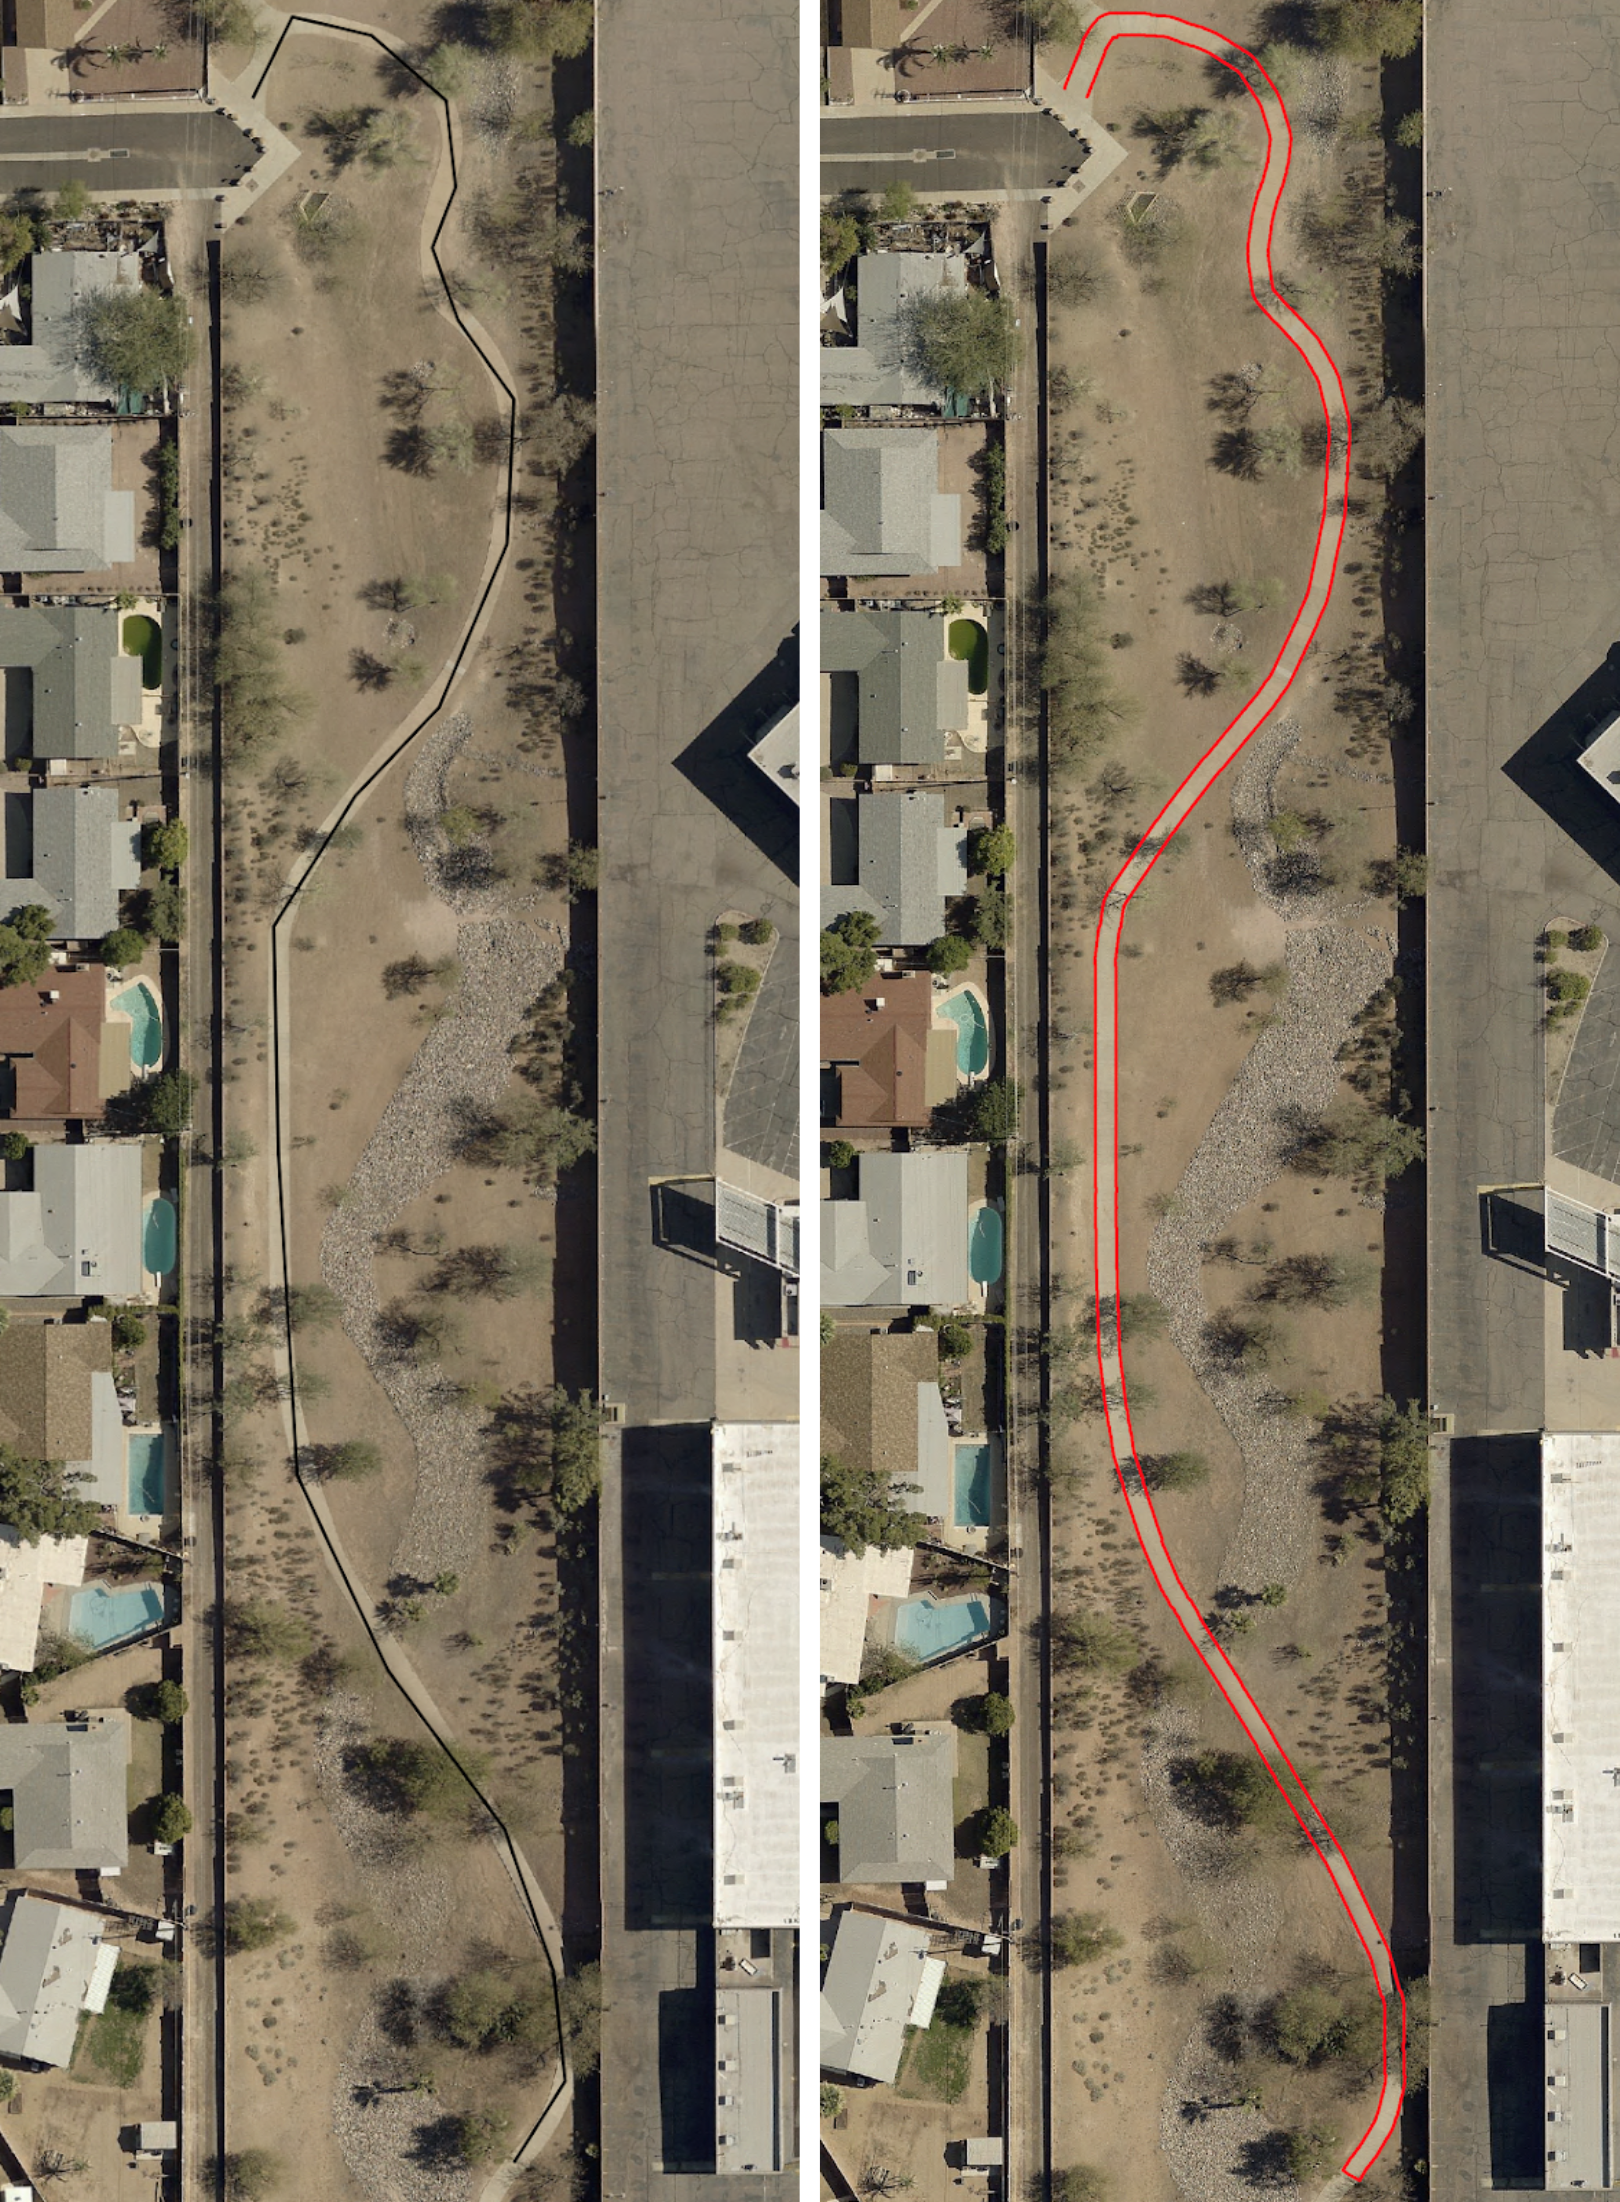
\includegraphics[width=0.85\textwidth]{Figures/Goal.png} 
\caption[Objective Demonstration]{
A demonstration  on input data and output result. 
With the input map and initial trajectory (left), 
we estimate detailed boundaries(right) with our \ac{DP} approach. 
The trajectory is marked in black and the boundaries are marked in red. 
We output the edges information as a .geojson file.}
\label{fig:goal} 
\end{figure}


Public domain or crowd-sourced repositories of spatial data such as \ac{OSM}~\cite{OpenStreetMap} represent a very
complete and frequently updated source of information which includes street vector data, and to a much lesser extent,
the locations of walking paths (called foot-ways by \ac{OSM}). However, the data is acquired from a variety of sources that may not be registered with
enough precision to accurately place thin features such as walking paths. For thin structures such as sidewalks that are
visible in \ac{VHR} imagery, even small discrepancies between the digitized pathways and the imagery can be distracting
when used to visualize an overlaid map. As new \ac{VHR} aerial imagery becomes available thin features such as walking
paths are discernible with higher precision, but ortho-rectification processes may not precisely align the imagery with
previously digitized features.

% \todo[]{show result with initial trajectory is off}

In addition, poorly registered walking paths could confound any algorithm that might hope to automatically locate
features on the path including obstacles, damage, overgrowth, or stairways that could impact the walkability. Several
authors\cite{femiani2009interval, femiani2007road} have worked on segmenting streets and sidewalks or other linear
features directly from aerial imagery; however sidewalks are much thinner than streets and are often partially occluded.
More importantly, these methods are mainly concerned with the connectivity of the extracted pathways and not with
identifying the precise boundaries. 

The problem we solve is illustrated in Figure \ref{fig:goal}.  We are given an input orthorectified image with an
initial trajectory (left) and we aim to find a ribbon (right). The initial trajectory is drawn in black, and boundaries 
of the ribbon are drawn in in red. 
Figure \ref{fig:fw_ov} demonstrates a step by step  diagram of our approach, 
from the input map (a), along with the initial
trajectory (b), we generate the ribbon-image with the given medial-curve (c).
We generate an initial estimation for the likelihood of each
pixel (d) with along the ribbon-image, then apply our \ac{DP} solution (e)
 to find a \ac{MAP} estimate of the ribbon.
Our approach, which we call \ac{DPRST}, can be used to refine the trajectories or recover the thickness of 
walking paths or other ribbon-like features. 
%
%Several automatic approaches model segmentation as a \ac{CRF} in order to ensure that the resulting output
%configurations are plausible \cite{ActiveContou09, Rother2004-ou, Achanta:149300}.

\begin{figure}[H] 
\centering 
\includegraphics[width=\textwidth]{Figures/diagram.png} 
\caption[Framework Demonstration]{
Our approach adopted to predict precise boundaries for ribbon-like features. 
The black line strip indicates a sidewalk's geometric information, 
and red lines show the identified ribbon boundaries. 
From top-left to bottom-right we show:
(a)~the input map, 
(b)~initial trajectory, 
(c)~the warped ribbon image, 
(d)~density estimation for the likelihoods of pixels, 
(e)~the result from our \ac{DP} solution, 
(f)~the result after reshaping sidewalk.} 
\label{fig:fw_ov} 
\end{figure}

\section{Challenges}\label{sec:challenges}

\begin{figure}[H] 
\centering 
\includegraphics[width=0.75\textwidth]{Figures/Challenge.png} 
\caption[Challenges Demonstration]{
A demonstration of some challenges faced by in our approach. From left to right, top to
bottom, it shows 
a sidewalk whose appearance is interrupted by shadow,
camouflage with adjacent materials,
and blocked by obstacles.}
\label{fig:challenge_demo}
\end{figure}

As shown in figure \ref{fig:challenge_demo}, the main challenge addressed by our approach is to predict precise
boundaries for ribbon-like walking paths when they are:

\begin{itemize} 
\item blocked by obstacles, 
\item under the shadow of trees, cars, buildings, 
\item camouflage with adjacent materials (e.g. driveways, gutters),
\item partially damaged so texture varies along the sidewalk.
\end{itemize}

Under these circumstances, most feature segmenting tools will not able to locate accurate boundaries, their results may
recognize the non-sidewalk pixels as the sidewalk or the other way around.

\section{Contributions}\label{sec:contributions}

The aim of this work is to precisely align and determine the width of a coarsely registered ribbon-like feature to match
its appearance in a \ac{VHR} image. The input is a \ac{VHR} georeferenced and orthorectified image along with a set of
linear features that are close to, but perhaps not precisely aligned with the center of a ribbon-like feature. In
particular, we expect that the ribbon will be made of a material with a somewhat uniform appearance (e.g. asphalt,
gravel, or concrete) but that its appearance will be affected by shadows and interrupted by occlusions from vegetation,
pedestrians, or vehicles such as bicycles. Our aim is to determine a more precise mid-line and an estimate for the width
of the ribbon-like feature, which can vary slowly along its trajectory. The solution proposed in this paper does not
rely on prior knowledge of the material on or around the ribbon, but instead, it estimates material appearance based on
on the initial trajectory. We
refine the placement of an initial estimate for the ribbon's mid-line with a shape-based prior that favors a result with little 
change in direction (bending) of the medial trajectory, and that favors small changes in thickness.

Our contributions are as follows: 
\begin{itemize} 
\item We introduce a \textit{Ribbon Prior} for segmenting linear feature that have slowly varying
      width and smooth (low curvature) medial trajectories. 
\item A novel \ac{DP} approach is proposed for aligning ribbon-like features to orthoimagery. 
    We do not require large training sets; a few parameters to control the smoothness of
	the resulting ribbon along with a coarse initial estimate of the trajectory are all that is needed. 
	Unlike
	methods that aim to recover the trajectories only, in our approach a likely thickness is directly identified so that
	more plausible trajectories and boundaries can be identified. 
\item An application to the problem of registering
	sidewalks to aerial photographs is demonstrated, allowing \ac{GIS} data sets to be improved as high-resolution ortho
	imagery becomes available. 
\end{itemize}